\documentclass[crop]{standalone}

\usepackage{amsmath}

\usepackage[dvipsnames]{xcolor}
\usepackage{tikz}

\usetikzlibrary{shapes,decorations,arrows,calc,arrows.meta,fit,positioning}
\tikzset{
    -latex,
    node distance =1 cm and 1 cm,
    semithick,
    O/.style ={rounded rectangle, draw, minimum width = 0.7 cm},
    U/.style ={rounded rectangle, draw, minimum width = 0.7 cm, dashed},
    fontscale/.style = {font=\huge}
}

\begin{document}


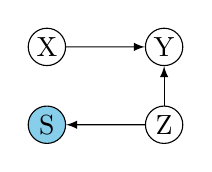
\begin{tikzpicture}
  \node[O] (x) at (0,0) {X};
  \node[O] (y) [right =of x] {Y};
  \node[O] (z) [below =0.5cm of y] {Z};
  \node[O, fill=SkyBlue] (s) [left =of z] {S};
  \path (x) edge (y);
  \path (z) edge (y);
  \path (z) edge (s);

\end{tikzpicture}


\end{document}
